\documentclass[french, 12pt, aspectratio=2013]{beamer} 
% valeur possibles : article, proc, book, report, letter, slides
% options possibles : twosides (recto-verso), 12pt, 11pt, ... (taille de police), draft (brouillon)

% Language setting
% Replace `english' with e.g. `spanish' to change the document language
\usepackage[french]{babel}
\usepackage[T1]{fontenc}
\usepackage{amssymb}
\usepackage{shadowtext}

% Useful packages
\usepackage{amsmath}
\usepackage{graphicx}

%tableau pleine largeur
\usepackage{tabularx}

%faire des dessins
\usepackage{tikz}

\usepackage{algorithm}

%\usepackage{fourier}
\usepackage{fontawesome}

\usepackage{color}
\newcommand{\md}[1]{\textcolor{cyan}{#1}}
\newcommand{\alh}[1]{\textcolor{teal}{#1}}

\newcommand{\append}{\texttt{append }}
\newcommand{\prepend}{\texttt{prepend }}
\newcommand{\replace}{\texttt{replace }}
\newcommand{\fullreplace}{\texttt{full\_replace }}



% Source - https://tex.stackexchange.com/a/680027
% Posted by C.F.G
% Retrieved 2026-08-27, License - CC BY-SA 4.0

\newenvironment<>{violetblock}[1]{%
    \setbeamercolor{block title}{fg= violet!80!black,bg= violet!40!white}%
    %\setbeamerfont{block title example}{family=\ssfamily}
    \begin{block}{#1}{#2}}{\end{block}}


\usepackage[dvipsnames]{xcolor}


\usepackage{listings}

\usepackage{appendixnumberbeamer}

% Theme choice:
\usetheme{Boadilla}


\AtBeginSection[]{
    \begin{frame}{Sommaire}
        \tableofcontents[currentsection]
    \end{frame}
}


\title{Interprétabilité Mécaniste pour l’Extraction d’Information dans les systèmes de RAG}
\author{Marine DELVALLEZ}

\setbeamertemplate{footline}[frame number]
\setbeamertemplate{navigation symbols}{}
\defbeamertemplate*{headline}{}
{%
  \setbeamercolor{subsection in head/foot}{fg=white}
  \begin{beamercolorbox}{section in head/foot}
    \insertsectionnavigationhorizontal{\paperwidth}{}{}
    \insertsubsectionnavigationhorizontal{\paperwidth}{}{}
  \end{beamercolorbox}%
 }


\begin{document}
\addtocounter{framenumber}{-1}
\begin{frame}[plain]
        
\includegraphics[scale=0.3]{images/Logo Minerve_RVB.jpg} \hfill
        
\includegraphics[scale=0.2]{images/France_2030_Logo_rouge_bleu_transparent.png} \hfill
        
\includegraphics[scale=0.3]{images/LIFO.png}
        \centering
        \Large Interprétabilité Mécaniste pour l’Extraction d’Information dans les systèmes de RAG\\
        \large Soutenance de stage de Master 2\\
        
        \vfill %\vspace{3mm}
        \normalsize Marine DELVALLEZ \hfill
        \textit{Master 2 Informatique GPEx Minerve}\\
        \vfill %\vspace{3mm}
        \small
        \begin{tabular}{llll}
            \emph{Jury} : & Thi-Bich-Hanh DAO &\emph{Tutrice de stage} : & Anaïs HALFTERMEYER\\
                          & Anaïs HALFTERMEYER &                        & \\
                          & Marie HÉNAULT
        \end{tabular}
        \vfill %\vspace{3mm}
        \centering \footnotesize 2 Septembre 2026 \\
    \end{frame}

\begin{frame}{Sommaire}
    \tableofcontents[]
\end{frame}

%%%%%%%%%%%%%%%%%%%%%%%%%%%%%%%%%%%%%%%%%%%%%%%%%%%%%%%%%%%%%%%%%%%%%%
\section{État de l'art}
    \subsection{Retrieval Augmented Generation - RAG}
        \begin{frame}{Retrieval Augmented Generation - RAG \cite{lewis_retrieval-augmented_2020}}
            %\md{Définiton de RAG, Schéma de l'architecture de base, tâches et sous-tâche d'IR}

            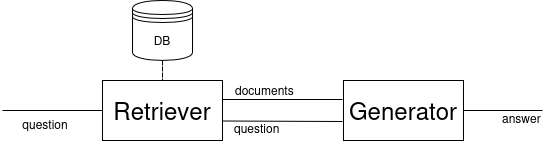
\includegraphics[width=\textwidth]{images/DefRAG.drawio.png}
            \pause
            \begin{columns}
                \begin{column}{0.45\textwidth}
                    \begin{block}{Tâches du RAG}
                        \begin{itemize}
                            \item Question Answering
                            \item Fact Checking
                            \item Dialogue
                        \end{itemize}
                    \end{block}
                \end{column}
                \pause
                \begin{column}{0.45\textwidth}
                    \begin{block}{Sous-tâches}
                        \begin{itemize}
                            \item \textbf<4>{Extraction de document}/ d'information
                            \item Synthèse
                            \item Génération de texte
                        \end{itemize}
                    \end{block}
                    
                    
                \end{column}
\end{columns}
        \end{frame}
        
        
    \subsection{Explicabilité pour le RAG}
        \begin{frame}{Explicabilité de l'IA et RAG}
            %\md{XAI > XRAG > XIR : On retrouve les problèmes classiques du DL dans le RAG. Le RAG se divisant en deux composants, on distingue XIR, XGen et Mise en commun. On se concentre sur XIR}

            \begin{alertblock}{}
                On a besoin d'expliquer les systèmes RAG !
            \end{alertblock}
            {\footnotesize \cite{fan_survey_2024}}
            \begin{picture}(370,170)
                \put(0,65){\onslide<1>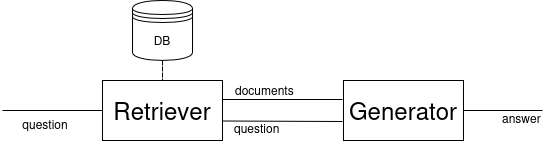
\includegraphics[width=\textwidth]{images/DefRAG.drawio.png}}
                \put(0,65){\onslide<2>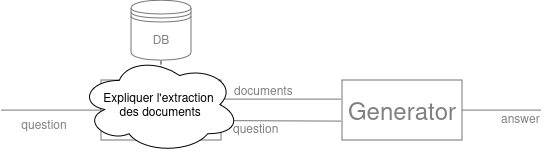
\includegraphics[width=\textwidth]{images/XRAG/XRAG_step1.drawio.png}}
                \put(0,65){\onslide<3>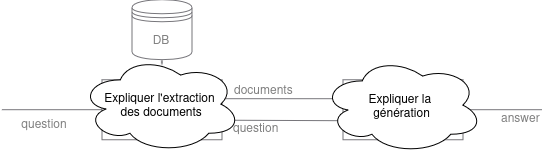
\includegraphics[width=\textwidth]{images/XRAG/XRAG_step2.drawio.png}}
                \put(0,0){\onslide<4>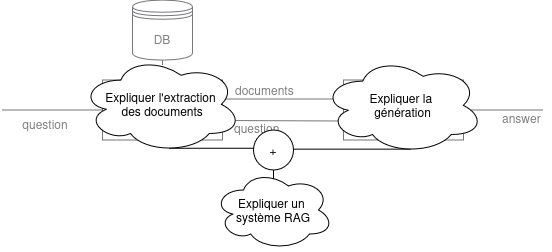
\includegraphics[width=\textwidth]{images/XRAG/XRAG_step3.drawio.png}}
                \put(0,0){\onslide<5>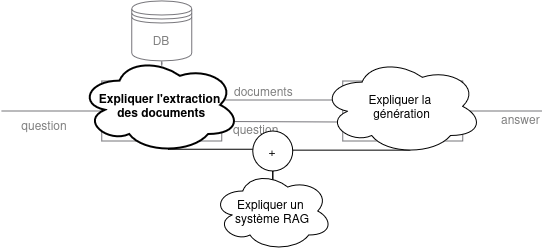
\includegraphics[width=\textwidth]{images/XRAG/XRAG_step4.drawio.png}}
            \end{picture}
            
        \end{frame}

        \begin{frame}{Explicabilité de l'IA et Interprétabilité Mécaniste \cite{somvanshi_bridging_2026}}
            %\md{Définition et situer InterpMech, taxonomie de \cite{somvanshi_bridging_2026}}

            \begin{center}
                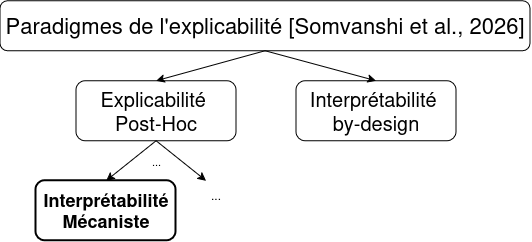
\includegraphics[width=0.65\textwidth]{images/InterprétabiliteMechaniste_Somvanshi-et-al_2026.drawio.png}
            \end{center}
            \pause
            \begin{block}{Interprétabilité Mécaniste}
                Explorer les \textbf{activations des composants} du modèle pour \textbf{identifier ceux qui provoquent ou influencent} un comportement cible
            \end{block}
            
        \end{frame}

        \begin{frame}{Interprétabilité Mécaniste \cite{somvanshi_bridging_2026}}
            %\md{Définition et situer InterpMech, taxonomie de \cite{somvanshi_bridging_2026}}

            \begin{block}{Interprétabilité Mécaniste }
                Explorer les \textbf{activations des composants} du modèle pour \textbf{identifier ceux qui provoquent ou influencent} un comportement cible
            \end{block}

            Plusieurs approches:

            \begin{itemize}
                \item Manual Circuit Tracing
                \item Representation Analysis
                \item Toy Models and Synthetic Tasks
                \item \textbf<2>{Intervention-based Techniques} 
                \pause 
                \begin{itemize}
                    \item Activation Patching
                    \item ...
                \end{itemize}
            \end{itemize}
            
        \end{frame}

        \begin{frame}{Activation Patching pour l'IR \cite{chen_axiomatic_2024} : intuition }
            %\md{intuition du fonctionnement de AP (animation utilisée au séminaire), évocation de MechIR comme implémentation}
            
            \begin{picture}(350,150)
                \put(0,0){\onslide<1>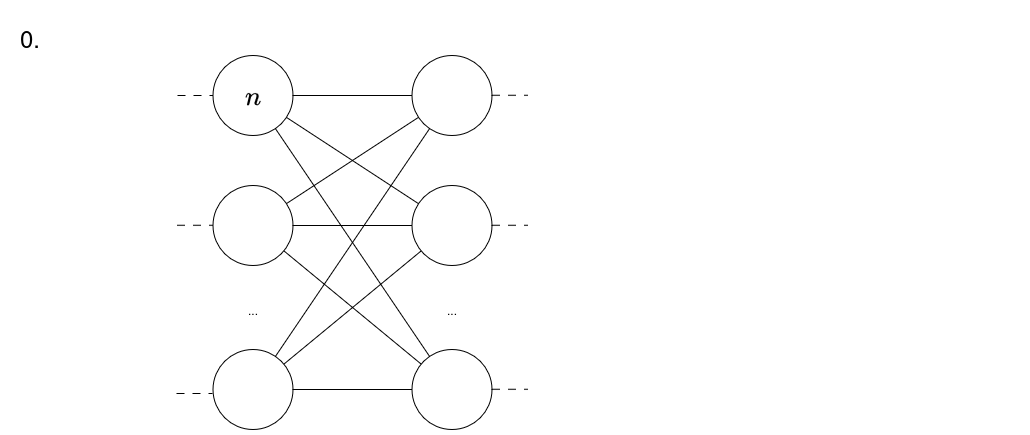
\includegraphics[width=\textwidth]{images/activationpatching/Step0_ActivationPatching.drawio.png}}
                \put(0,0){\onslide<2>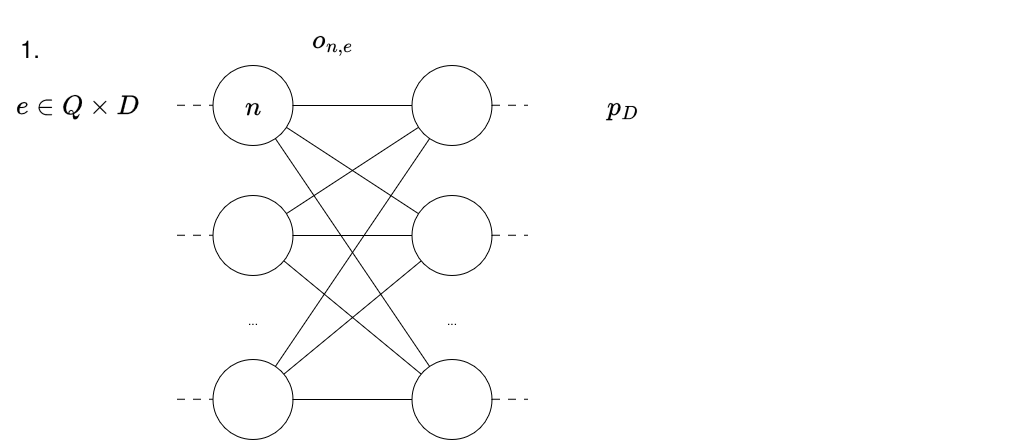
\includegraphics[width=\textwidth]{images/activationpatching/Step1_ActivationPatching.drawio.png}}
                \put(0,0){\onslide<3>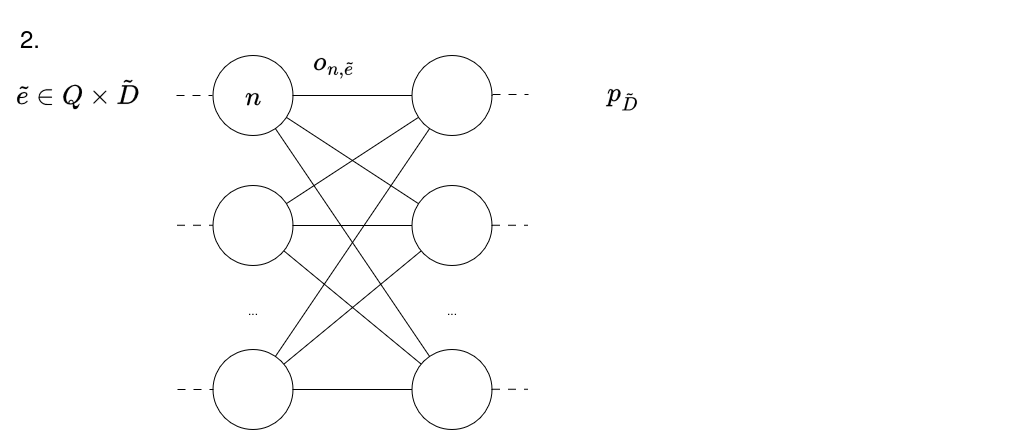
\includegraphics[width=\textwidth]{images/activationpatching/Step2_ActivationPatching.drawio.png}}
                \put(0,0){\onslide<4>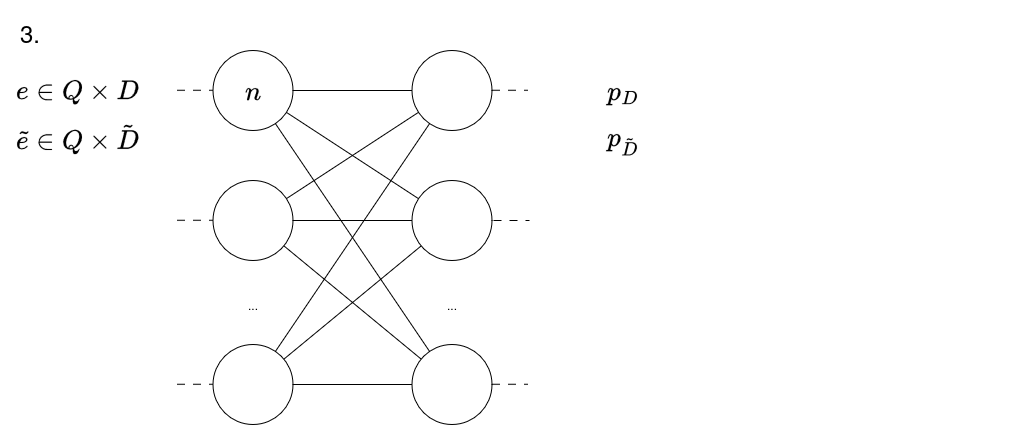
\includegraphics[width=\textwidth]{images/activationpatching/Step3_ActivationPatching.drawio.png}}
                \put(0,0){\onslide<5>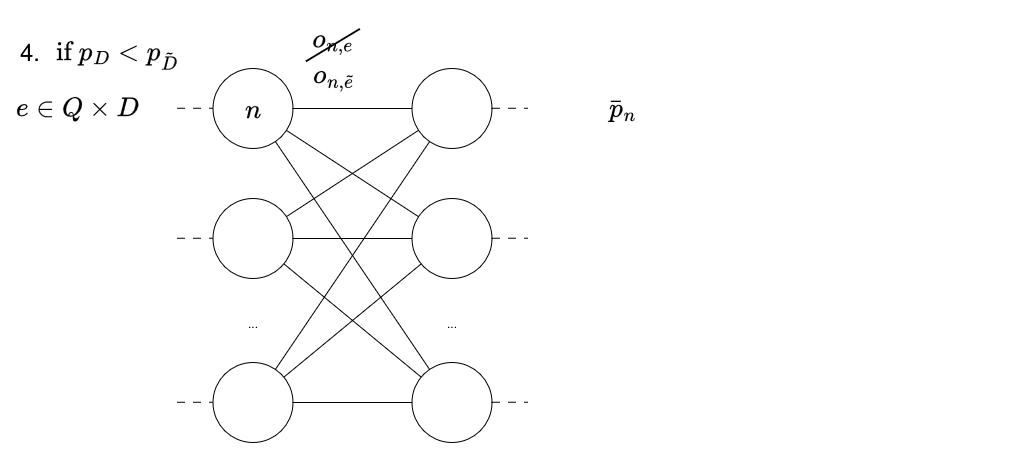
\includegraphics[width=\textwidth]{images/activationpatching/Step4_ActivationPatching.drawio.png}}
                \put(0,0){\onslide<6->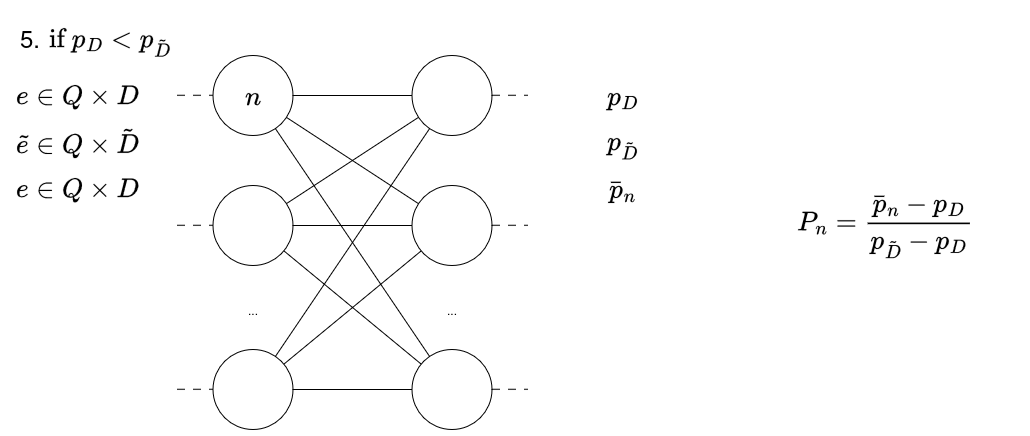
\includegraphics[width=\textwidth]{images/activationpatching/Step5_ActivationPatching.drawio.png}}
            \end{picture}
            

            
            %\onslide<7>{MechIR \cite{parry_mechir_2025} permet d'implémenter l'activation patching}
        \end{frame}
        
%%%%%%%%%%%%%%%%%%%%%%%%%%%%%%%%%%%%%%%%%%%%%%%%%%%%%%%%%%%%%%%%%%%%%%  
\section{Objectifs de ce stage}
        \begin{frame}{Hypothèses et Objectifs}
            %\md{slide hypothèses et objectifs issue de présentation du séminaire + remis au goût du jour}
            \begin{block}{Langue de spécialité \cite{cabre_terminologie_1998}}
                Ensemble de sous-codes linguistiques spécifiques à un domaine de spécialité (lexique, syntaxe,...)
            \end{block}
            \begin{block}{Hypothèses}
                \begin{description}
                    \item[H1 :] Le vocabulaire de spécialité (lexique) repose sur certains composants du modèle
                    \item[H2 :] L'activation patching permet de les localiser
                \end{description}
            \end{block}
            \begin{block}{Objectifs}
                \begin{itemize}
                    \item Appliquer l'activation patching à la localisation du vocabulaire de spécialité de la \textit{défense}
                    \item Proposer une méthodologie d'utilisation de MechIR
                \end{itemize}
                
            \end{block}
        \end{frame}

%%%%%%%%%%%%%%%%%%%%%%%%%%%%%%%%%%%%%%%%%%%%%%%%%%%%%%%%%%%%%%%%%%%%%%
\section{Préliminaires}
        \begin{frame}{Cas d'application}
            \begin{figure}
                \centering
                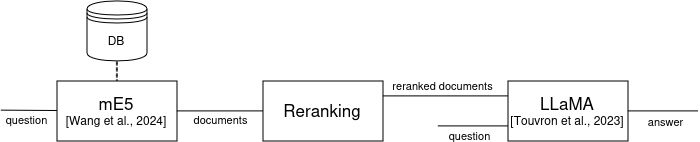
\includegraphics[width=0.8\textwidth]{images/RAGHN-perso.drawio.png}
                 \caption{Version simplifiée de RAG4HistoricalNewspapers \cite{tran_retrieval_2024}}
            \end{figure}
            \begin{columns}
                \begin{column}{0.45\textwidth}
                    \begin{block}{mE5-small \cite{wang_multilingual_2024}}
                        \begin{itemize}
                            \item $\approx 17 M$ de paramètres
                            \item encodeur-only
                            \item bi-encodeur
                        \end{itemize}
                    \end{block}
                \end{column}
                \pause
                \begin{column}{0.45\textwidth}
                    \begin{block}{MechIR \cite{parry_mechir_2025}}
                        \begin{itemize}
                            \item Alternative à TransformerLens \cite{nanda_transformerlens_2022} pour les encodeur-only
                            \item Implante des outils pour l'Activation Patching
                        \end{itemize}
                        
                    \end{block}
                \end{column}
            \end{columns}
        \end{frame}

        \begin{frame}{Dataset}
            %\md{Présentation du format et statistiques du dataset (1Q, 28 docs, 50\% pertinent, }

            \begin{columns}
                \begin{column}{0.6\textwidth}
                    \begin{block}{Contenu thématique}
                        \begin{itemize}
                            \item Extraits de documents issus des données du challenge RAG@EvalLLM
                            \item Question sur les \textit{limitations techniques des systèmes de drones}
                            \item Trois documents
                            \begin{itemize}
                                \item Limitations techniques du drone
                                \item Matériel de guerre - Code de la défense
                                \item Fausses informations pendant les JO/JP
                            \end{itemize}
                        \end{itemize}
                    \end{block}
                \end{column}
                \begin{column}{0.30\textwidth}
                    \begin{block}{Structure}
                        \begin{itemize}
                            \item 1 question
                            \item 28 extraits
                            \item 50\% de documents pertinents
                        \end{itemize}
                    \end{block}
                \end{column}
            \end{columns}
            

            
        \end{frame}

%%%%%%%%%%%%%%%%%%%%%%%%%%%%%%%%%%%%%%%%%%%%%%%%%%%%%%%%%%%%%%%%%%%%%%
\section{Expérimentations}
    \subsection{Construction des perturbations}
        \begin{frame}{Construire des perturbations}
            \begin{violetblock}{Qu'est-ce qu'une bonne perturbation ?}
                \begin{itemize}
                    \item Modification minimale du document \cite{chen_axiomatic_2024}
                    \item Modification significative de la sortie \cite{chen_axiomatic_2024}
                    \item Grande couverture du dataset
                \end{itemize}
            \end{violetblock}
            \begin{block}{Perturbations proposées par \cite{parry_mechir_2025}}
                \begin{description}
                    \item[\prepend] : ajouter un mot au début du document
                    \item[\append] : ajouter un mot à la fin du document
                    \item[\replace] : remplacer un mot par un autre
                \end{description}
            \end{block}
            \pause
            \underline{Exemple} : remplacer \textit{aérien} par \textit{poétique}
            \begin{overlayarea}{13cm}{8mm}
                \only<2> {\textit{\quad Certaines limitations sont plus particulièrement liées aux caractéristiques du vecteur aérien}}
                \only<3-> {\textit{ \quad Certaines limitations sont plus particulièrement liées aux caractéristiques du vecteur \textbf{poétique}}}
            \end{overlayarea}
        \end{frame}
        \begin{frame}{Choisir le mot à remplacer}
            %\md{Les indicateurs proposés pour identifier les mots à remplacer}
            \begin{columns}
                \begin{column}{0.45\textwidth}
                    \begin{block}{Critères de choix des mots}
                        \begin{itemize}
                            \item Fréquence dans le dataset
                            \item TF-IDF du mot dans le dataset
                            \item Présence du mot dans la question
                            \item Porteur d'un sens marqué
                            \item \textbf{Appartenance à au moins un autre sous-code}
                        \end{itemize}
                    \end{block}
                \end{column}
                \pause
                \begin{column}{0.5 \textwidth}
                    \fontsize{10}{0.8\baselineskip}\selectfont
                    \begin{tabular}{|l|l|l|}
                    \hline
                        Mot & Fréquence & TF-IDF \\ \hline \hline
                        \textbf{matériel} & 16 & 0.063 \\ \hline
                        \textbf{système} & 11 & 0.054 \\ \hline
                        \textbf{limitation} & 6 & 0.050 \\ \hline
                        \textbf{drone} & 10 & 0.044 \\ \hline
                        \textbf{défense} & 10 & 0.044 \\ \hline
                        prendre & 6 & 0.043 \\ \hline
                        compte & 5 & 0.040 \\ \hline
                        action & 8 & 0.040 \\ \hline
                        \textbf{article} & 9 & 0.040 \\ \hline
                        ministre & 8 & 0.039 \\ \hline
                        \textbf{aérien} & 7 & 0.037 \\ \hline
                        acteur & 6 & 0.034 \\ \hline
                        guerre & 8 & 0.034 \\ \hline
                        informationnel & 5 & 0.031 \\ \hline
                        information & 6 & 0.030 \\ \hline
                    \end{tabular}
                \end{column}
            \end{columns}
        \end{frame}

        \begin{frame}{Choisir le mot remplaçant}
            %\md{Les 4 niveaux de perturbation, tableau du rapport revisité}
            \fontsize{10}{0.8\baselineskip}\selectfont
            Étant donné le mot cible (à remplacer)
            \begin{tabular}{|c||p{0.30\linewidth}|p{0.25\linewidth}|p{0.25\linewidth}|}
                \hline
                Niv & Mot remplaçant & Phénomène cible & Exemple \\ \hline  \hline
                1 & Synonyme dans la langue de spécialité & Localisation du mot remplacé & aérien $\to$ de vol\\ \hline
                2 & Synonyme dans le langage courant & Localisation du sens & aérien $\to$ poétique \\ \hline
                \pause
                3 & Mot sémantiquement incompatible & Localisation du sens (sans réparation) & aérien $\to$ épicurien \\ \hline
                4 & Groupe de mots \textit{absurde} sémantiquement incompatibles & Localisation du sens (avec bruit) & aérien $\to$ acide tracté \\ \hline
            \end{tabular}
        \end{frame}

        \begin{frame}{Perturbation de type \fullreplace}
            %\md{définition, en quoi est-ce plus interessant (meilleure couverture du dataset)}
            \begin{block}{Perturbation \fullreplace}
                Appliquer une liste de perturbations \replace \textbf{simultanément}
            \end{block}
            \underline{Exemple} : 
            \begin{itemize}
                \item remplacer \textit{aérien} par \textit{poétique}
                \item remplacer \textit{limitation} par \textit{bornage}
            \end{itemize}
                \begin{overlayarea}{13cm}{8mm}
                    \only<1> {\textit{\quad Certaines limitations sont plus particulièrement liées aux caractéristiques du vecteur aérien}}
                    \only<2-> {\textit{ \quad Certaines \textbf{bornage}s sont plus particulièrement liées aux caractéristiques du vecteur \textbf{poétique}}}
                \end{overlayarea}
            \begin{block}{Buts}
                \begin{itemize}
                    \item Augmenter la couverture du dataset
                    \item Effet d'ensemble
                \end{itemize}
            \end{block}            
        \end{frame}

    \subsection{Évaluation d'une perturbation}
        \begin{frame}{Distribution des scores de pertinence des documents}
            %\md{évaluation proposée par \cite{parry_mechir_2025} : perturbation de la distribution des score de pertinence du document}
            \begin{block}{}
                Objectif : Distributions de scores différentes pour les documents et documents perturbés \cite{parry_mechir_2025}
            \end{block}
            \begin{center}
                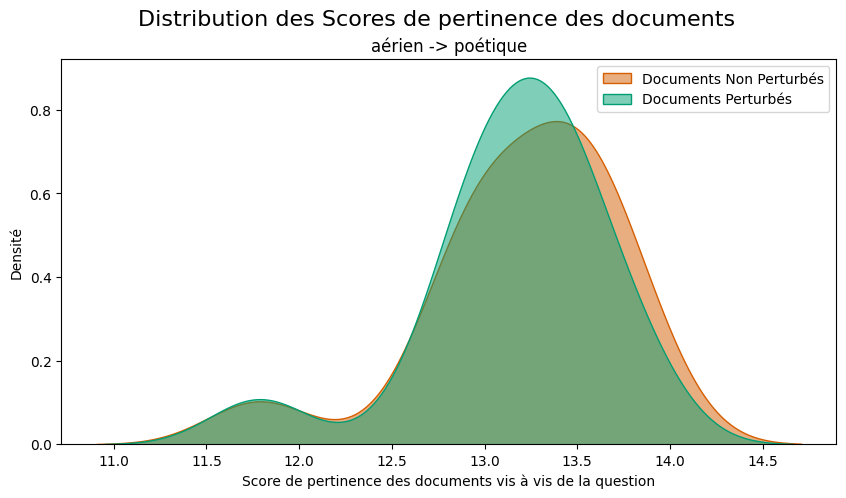
\includegraphics[width=0.6\textwidth]{images/DistribScoresPerturb_aerien-poetique.png}
            \end{center}
            \pause
            \textbf{Interprétation} :
                    Perte de pertinence d'une partie des documents
                
        \end{frame}

        \begin{frame}{En observant l'impact de la perturbation sur la question}
            \begin{block}{}
                Objectif : Estimer l'impact d'une perturbation sur  la question dans l'espace de représentation.
            \end{block}
            \begin{columns}
                \begin{column}{0.6\textwidth}
                    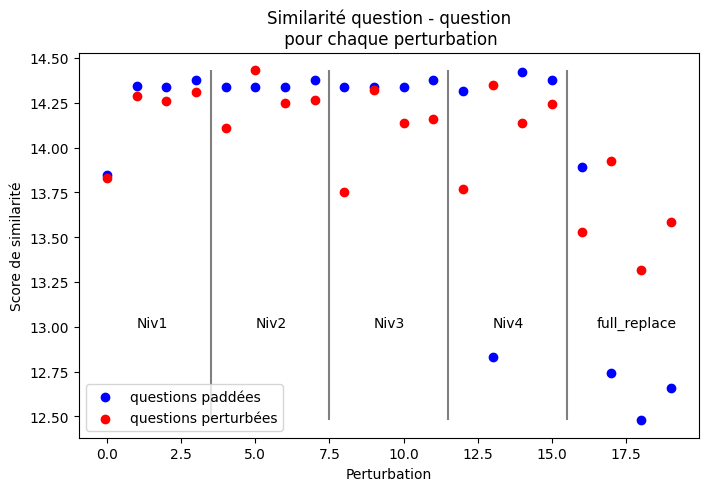
\includegraphics[width = \textwidth]{images/Exp9QuestioncommeDocument.png}
                \end{column}
                \begin{column}{0.4\textwidth}
                    \fontsize{10}{0.8\baselineskip}\selectfont
                    \textit{Quelles sont les trois principales catégories de limitations techniques affectant les systèmes de drones, et comment chacune influence-t-elle l'efficacité opérationnelle de ces vecteurs ?}
                    \begin{block}{Mots ciblés}
                        \begin{columns}
                            \begin{column}{0.5\textwidth}
                                \begin{itemize}
                                    \item drone
                                    \item limitation
                                \end{itemize}
                            \end{column}
                            \begin{column}{0.5\textwidth}
                                \begin{itemize}
                                    \item système
                                    \item technique
                                \end{itemize}
                            \end{column}
                        \end{columns}
                        
                    \end{block}
                \end{column}
            \end{columns}
        \end{frame}

        \begin{frame}{En séparant les documents pertinents et non-pertinents}
            \begin{block}{}
                Objectif : Identifier les documents perturbés et leur distribution en fonction de leur pertinence. 
            \end{block}
            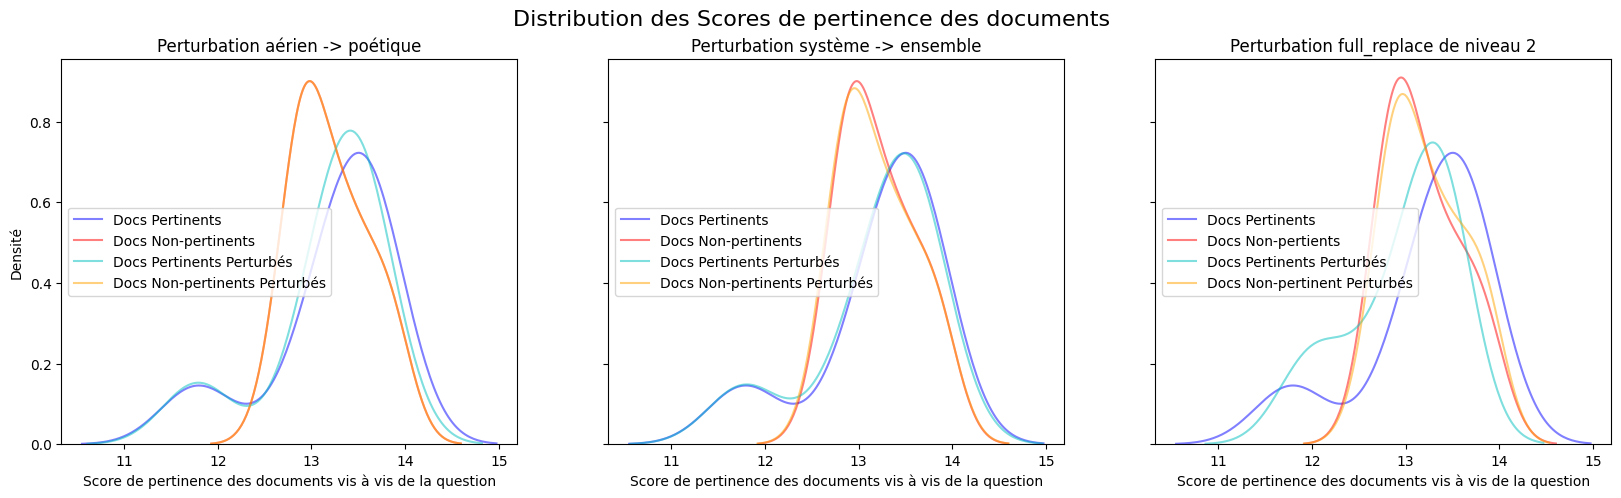
\includegraphics[width = \textwidth]{images/PerturbationScoreExemple_PosNeg.png}
            $\Rightarrow$ Répartition des mots ciblés biaisée 
        \end{frame}

        \begin{frame}{Confronter les perturbations entre elles}
            \begin{block}{}
                Objectif : Comparer l'impact des perturbations entre elles. Confirmer une progressivité. Choisir parmi plusieurs perturbations.
            \end{block}
            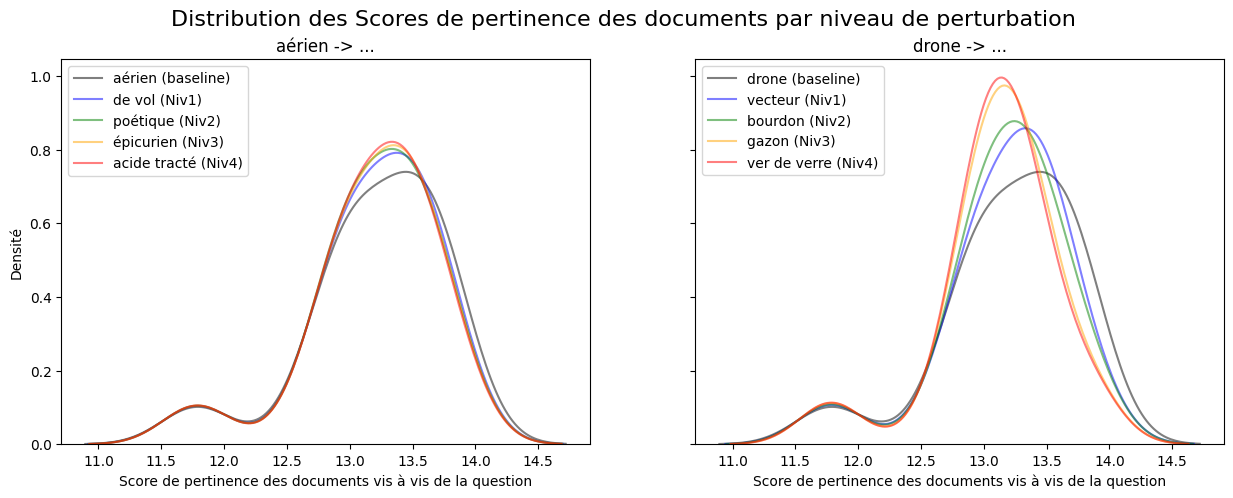
\includegraphics[width=\textwidth]{images/PerturbationScoreExemple_ParNiveaux.png}
        \end{frame}

    \subsection{Lecture des résultats de l'activation patching}

        \begin{frame}{Matrice de sensibilité}
            %\md{Exemple avec le graphique de \cite{parry_mechir_2025}. Ajoute des 4 autres graphiques + lecture accompagnée }
            \centering
            \begin{picture}(320,220)
                \put(0,110){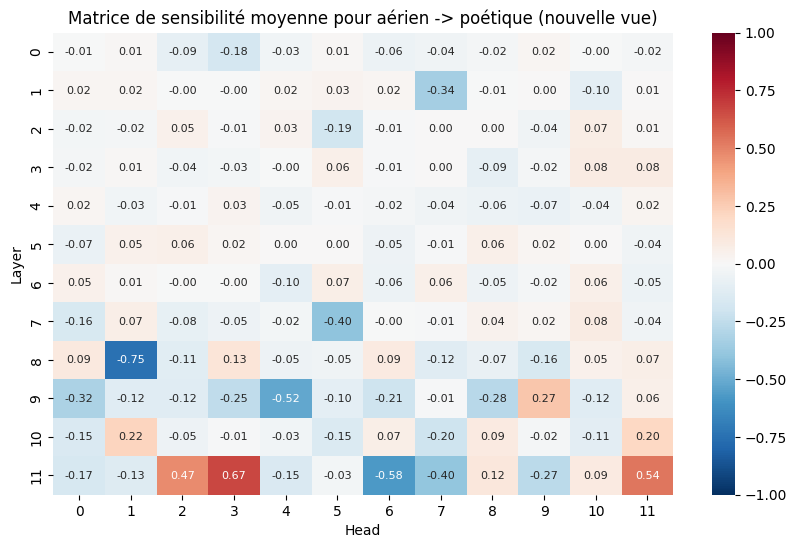
\includegraphics[width=0.4\textwidth]{images/MatriceSensibilite_new-mean_aerien-poetique.png}}
                \put(160,110){\onslide<2->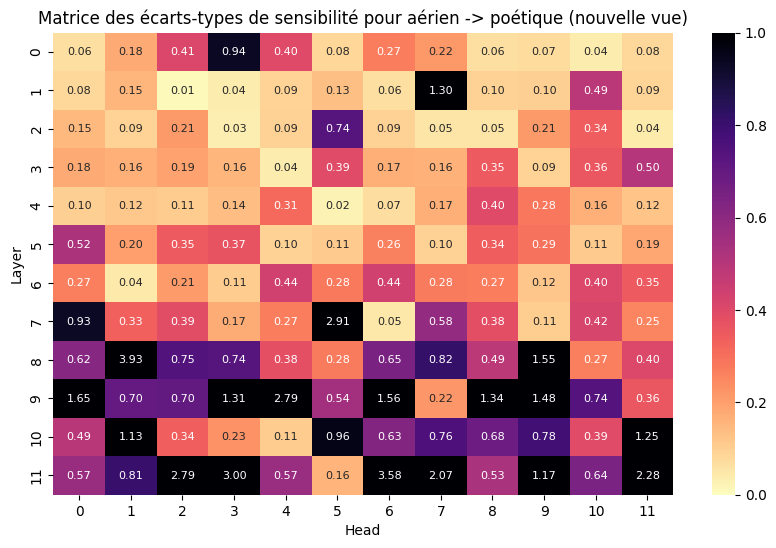
\includegraphics[width=0.4\textwidth]{images/MatriceSensibilite_new-std_aerien-poetique.png}}
                \put(0,0){\onslide<3->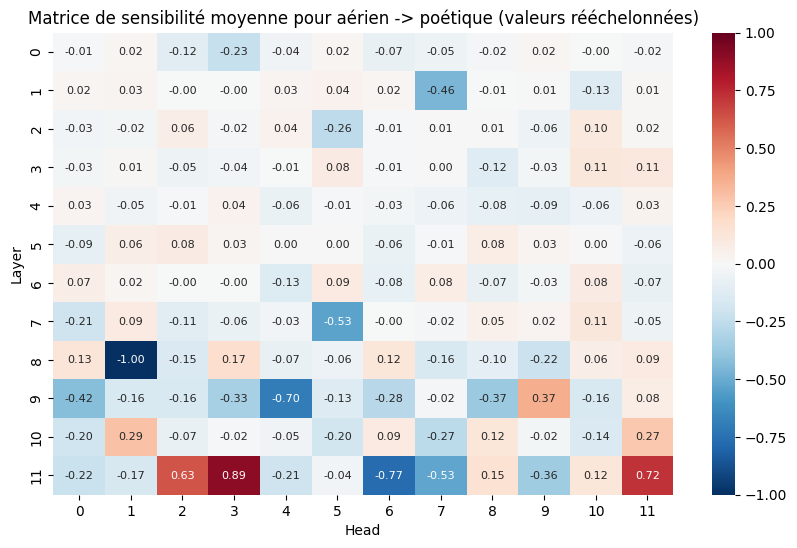
\includegraphics[width=0.4\textwidth]{images/MatriceSensibilite_resc-mean_aerien-poetique.png}}
                \put(160,0){\onslide<3->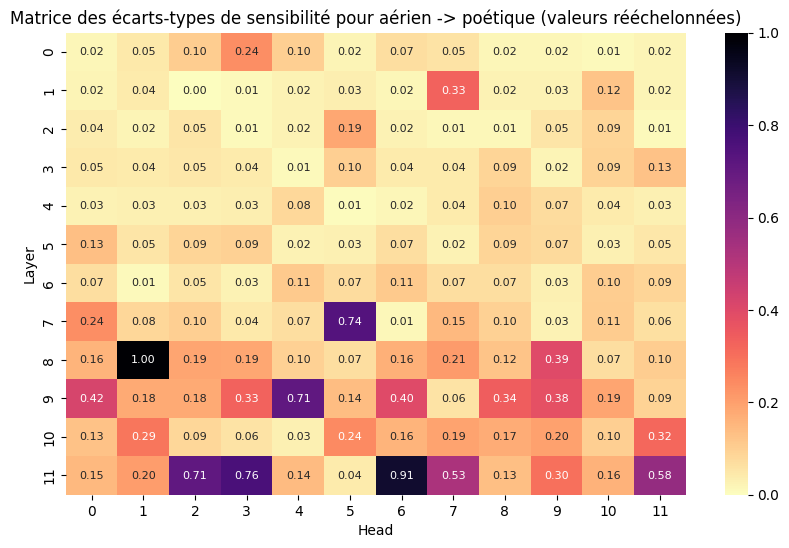
\includegraphics[width=0.4\textwidth]{images/MatriceSensibilite_resc-std_aerien-poetique.png}}
            \end{picture}
        \end{frame}

        \begin{frame}{Identification des noeuds sensibles}
            %\md{Construction du critère de sensibilité, matrice binaire pertinent ou non pour une perturbation (permet introduction progressive de la matrice ds noeuds sensibles)}
            \fontsize{10}{0.8\baselineskip}\selectfont
            \begin{violetblock} {Qu'est-ce qu'un noeud sensible?}
                \begin{itemize}
                    \item Sensibilité au patching forte
                    \item ... plus forte que les autres noeuds
                    \item ... pour certains documents
                \end{itemize}
            \end{violetblock}

            \begin{block}{Critère de sensibilité}
                $\left(\left(\mid mean \mid > 0.1\right) \wedge \left(\mid resc\_mean \mid > 0.5\right) \right) \vee \left( \left(std > 0.1\right) \wedge \left(resc\_std > 0.5\right)\right)$
            \end{block}

            \centering
            \begin{minipage}[c]{4.5cm}
                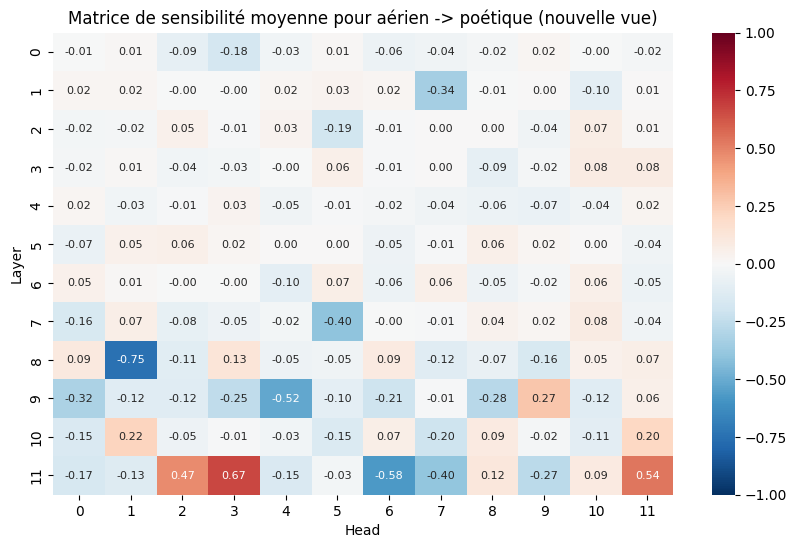
\includegraphics[width=\textwidth]{images/MatriceSensibilite_new-mean_aerien-poetique.png}
            \end{minipage}
            $\Rightarrow$
            \begin{minipage}[c]{4.5cm}
                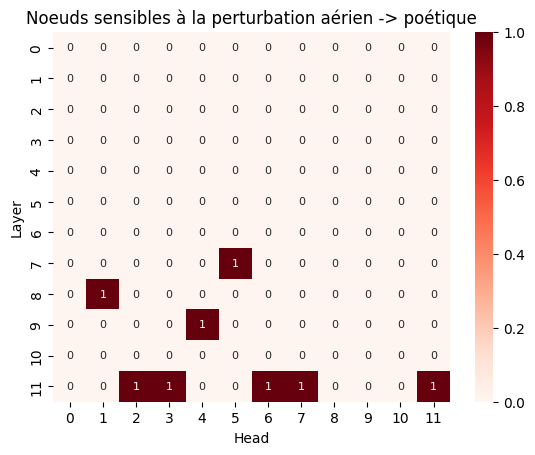
\includegraphics[width=0.8\textwidth]{images/MatNoeudsSensibles_aerien-poetique.png}
            \end{minipage}
            
        \end{frame}

        \begin{frame}{Matrice des noeuds sensibles}
            %\md{Visualisation de 2 matrices : perturbations ciblant un mot, perturbations d'un même niveau ~> pas toujours qqchose d’intéressant}

            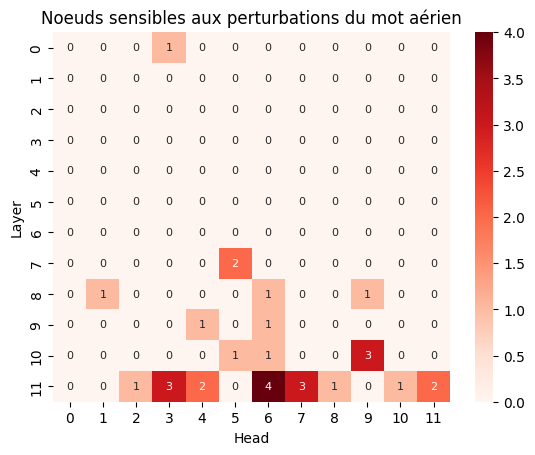
\includegraphics[width=0.49\textwidth]{images/NoeudsSensiblesAerien.png}
            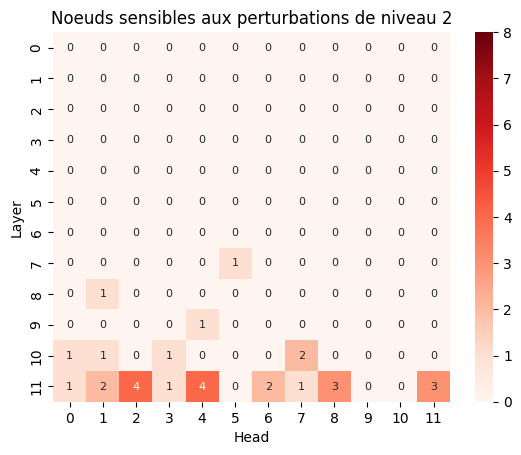
\includegraphics[width=0.49\textwidth]{images/NoeudsSensiblesNiv2.png}
            
        \end{frame}
    \subsection{Résultats}
        \begin{frame}{Résultats}
            \begin{block}{Quelques noeuds identifiés}
                \begin{columns}
                    \begin{column}{0.5\textwidth}
                        \begin{tabular}{|c|p{0.55\linewidth}|}
                            \hline
                            Mot / Niveau & Noeuds identifiés \\ \hline
                            article & (11,4) \\ \hline
                            aérien & (11,6), (11,3), (10,9) \\ \hline
                            drone & (11,4) \\ \hline
                            défense & (11,2) \\ \hline
                            matériel & (11,4), (11,9) \\ \hline
                        \end{tabular}
                    \end{column}
                    
                    \begin{column}{0.45\textwidth}
                        \begin{tabular}{|c|p{0.55\linewidth}|}
                            \hline
                            système & (11,1) \\ \hline
                            Niveau 3 & (11,3) \\ \hline
                            Niveau 4 & (1,7) \\ \hline
                            Full replace & (11,1), (11,5), (11,6), (11,3) \\ \hline
                        \end{tabular}
                    \end{column}
                \end{columns}
            \end{block}
            \pause
            \begin{block}{La méthodologie actuelle ...}
                \begin{itemize}
                    \item ... met en évidence des noeuds sensibles \textit{pour une perturbation}
                    \item ... met en évidence des noeuds sensibles \textit{pour un mot perturbé} (parfois)
                    \item ... ne met pas en évidence de tendance \textit{à l'échelle du vocabulaire}
                \end{itemize}
            \end{block}

        \end{frame}
        \begin{frame}{Analyse}
            \begin{violetblock}{\textbf{H1 :} Le vocabulaire de spécialité (lexique) repose sur certains composants du modèle}
                \begin{itemize}
                    \item On peut identifier une spécialisation de certains composants à l'échelle du mot
                    \item Sans savoir si elle relève du vocabulaire de spécialité, du mot ou du bruit
                \end{itemize}
                $\Rightarrow$ On ne peut pas conclure pour l'instant
            \end{violetblock}

            \begin{violetblock}{\textbf{H2 :} L'activation patching permet de les localiser}
                \begin{itemize}
                    \item L'activation patching permet de localiser les composants sensibles d'un modèle
                \end{itemize}
                $\Rightarrow$ On ne peut pas conclure
            \end{violetblock}

            %\md{reprendre les hypothèses et conclure dessus}
        \end{frame}

%%%%%%%%%%%%%%%%%%%%%%%%%%%%%%%%%%%%%%%%%%%%%%%%%%%%%%%%%%%%%%%%%%%%%%
\section{Conclusion et perspectives}
        \begin{frame}{À retenir}
            \begin{block}{Bonnes pratiques}
                \begin{itemize}
                    \item Perturbations couvrantes
                    \item Perturbations pertinentes (cas de \textit{article})
                    \item Vigilance et prise en compte des biais
                    \item Vigilance pour les noeuds de la dernière couche
                \end{itemize}
            \end{block}

            \begin{block}{Résultats}
                \begin{itemize}
                    \item L'activation patching permet de localiser les composants sensibles au sens de certains mots
                \end{itemize}
            \end{block}
        \end{frame}

        \begin{frame}{Perspectives d'amélioration}
            \begin{itemize}[<+->]
                \item Fonder et outiller l'échelle de niveau des perturbations \cite{greimas_semiotique_1979}
                \item Méthodologie pour mettre en perspective différents datasets
                \item Diversification des perturbations (\prepend, \append, ...)
                \item Étendre à la langue de spécialité
            \end{itemize}
        \end{frame}

        \begin{frame}{Intégration dans l'XRAG}
            %\md{lien avec le projet de thèse, projet dans lequel s'intègre le travail du stage, perspectives pour aller au bout de se projet}

            \begin{itemize}[<+->]
                \item Amélioration de la méthodologie
                \item Transformer les noeuds identifiés en cartographie
                \item Protocole d'extraction d'explication
                \item Rendre les explications accessibles à l'utilisateur non-informaticien
                \vspace{2mm}
                \item Protocole d'extraction d'améliorations
            \end{itemize}

        \end{frame}

        \begin{frame}{Conclusion sur les travaux du stage}
            %\md{liste à puce récap de ce qui a été présenté : Def de RAG, InterpMEch et AP + modèle et dataset challenge + Méthode de construction de peturbation +  outils de visualistaion des résultats de AP}

            \begin{itemize}
                \item Défrichage bibliographique
                \begin{itemize}
                    \item RAG et RA-LLM
                    \item Explicabilité pour le RAG et le RA-LLM
                    \item Interprétabilité mécaniste
                    \item Activation Patching
                \end{itemize}
                \item Challenge RAG@EvalLLM
                \begin{itemize}
                    \item Reprise d'un système RAG
                    \item Structuration itérative d'un dataset à la main
                \end{itemize} 
                \item Proposition d'une méthode d'utilisation de MechIR
                \item Proposition d'une méthode d'interprétation de l'activation patching
            \end{itemize}
        \end{frame}


%%%%%%%%%%%%%%%%%%%%%%%%%%%%%%%%%%%%%%%%%%%%%%%%%%%%%%%%%%%%%%%%%%%%%%
\appendix

\bibliographystyle{alpha} %apalike
\begin{frame}[allowframebreaks]{Références}
    \bibliography{sample.bib}
\end{frame}

\section{Annexes}

\begin{frame}{Activation Patching pour l'IR \cite{chen_axiomatic_2024}}
    \fontsize{10}{0.8\baselineskip}\selectfont % pour écrire plus petit en gardant l'interligne standard de beamer
    Soit $Q \times D \subset \mathcal{Q}\times\mathcal{D}$  l'ensemble des paires question, document. Soit $Q \times \tilde{D}$ le même ensemble mais avec les documents perturbés à la place 

                \begin{enumerate}
                    \item Faire une passe pour toutes les paires $Q\times D$
                    \begin{itemize}
                        \item noter $o_{n}^e$ la sortie de chaque nœud $n, \forall e \in Q\times D$
                        \item noter $p_D$ la performance du modèle sur les données non perturbées
                    \end{itemize} 
                    \item Faire une passe pour toutes les paires $Q\times \tilde{D}$
                    \begin{itemize}
                        \item noter $o_{n}^{\tilde{e}}$ la sortie de chaque nœud $n, \forall \tilde{e} \in Q\times \tilde{D}$
                        \item noter $p_{\tilde{D}}$ la performance du modèle sur les données perturbées
                    \end{itemize}
                    \item On renomme $D, e, \tilde{D}$ et $\tilde{e}$ respectivement
                    \begin{itemize}
                        \item $\hat{D}, \hat{e}, \check{D}$ et $\check{e}$ si $p_D > p_{\tilde{D}}$
                        \item $\check{D}, \check{e}, \hat{D}$ et $\hat{e}$ sinon
                    \end{itemize}
                    Pour chaque nœud $n$
                    \item Faire une passe de $Q\times\check{D}$ en remplaçant $o_{i,j}^{\check{e}}$ par $o_{n}^{\hat{e}}$ pour chaque $\check{e}$. On note la performance $\bar{p}_n$
                    \item $P_{n} = \frac{\bar{p}_n - p_{\hat{D}} }{p_{\check{D}} - p_{\hat{D}}}$ exprime l'impact de la perturbation sur la performance du modèle pour le nœud $n$
                \end{enumerate}
\end{frame}

\begin{frame}{Liste des perturbations pratiquées}
    \fontsize{10}{0.8\baselineskip}\selectfont
    \begin{tabular}{|l||l|l|l|l|}
            \hline
            Mot remplacé & Niveau 1 & Niveau 2 & Niveau 3 & Niveau 4 \\ \hline \hline
            aérien & de vol & poétique & épicurien & acide tracté \\ \hline
            article & sujet & déterminant & table & luge pontificale \\ \hline
            défense & protection & corne & fromage & poire retournée \\ \hline
            drone & vecteur & bourdon & gazon & ver de verre \\ \hline
            limitation & contrainte & bornage & animation & plastique anarchique \\ \hline
            matériel & outil & concret & post-it & porte sans poivre \\ \hline
            système & dispositif & ensemble & panneau & esperluette en vent \\ \hline
            technique & spécialisé & difficile & magique & feuille entubée \\ \hline
        \end{tabular}
\end{frame}

\begin{frame}[plain]{}
    \centering
    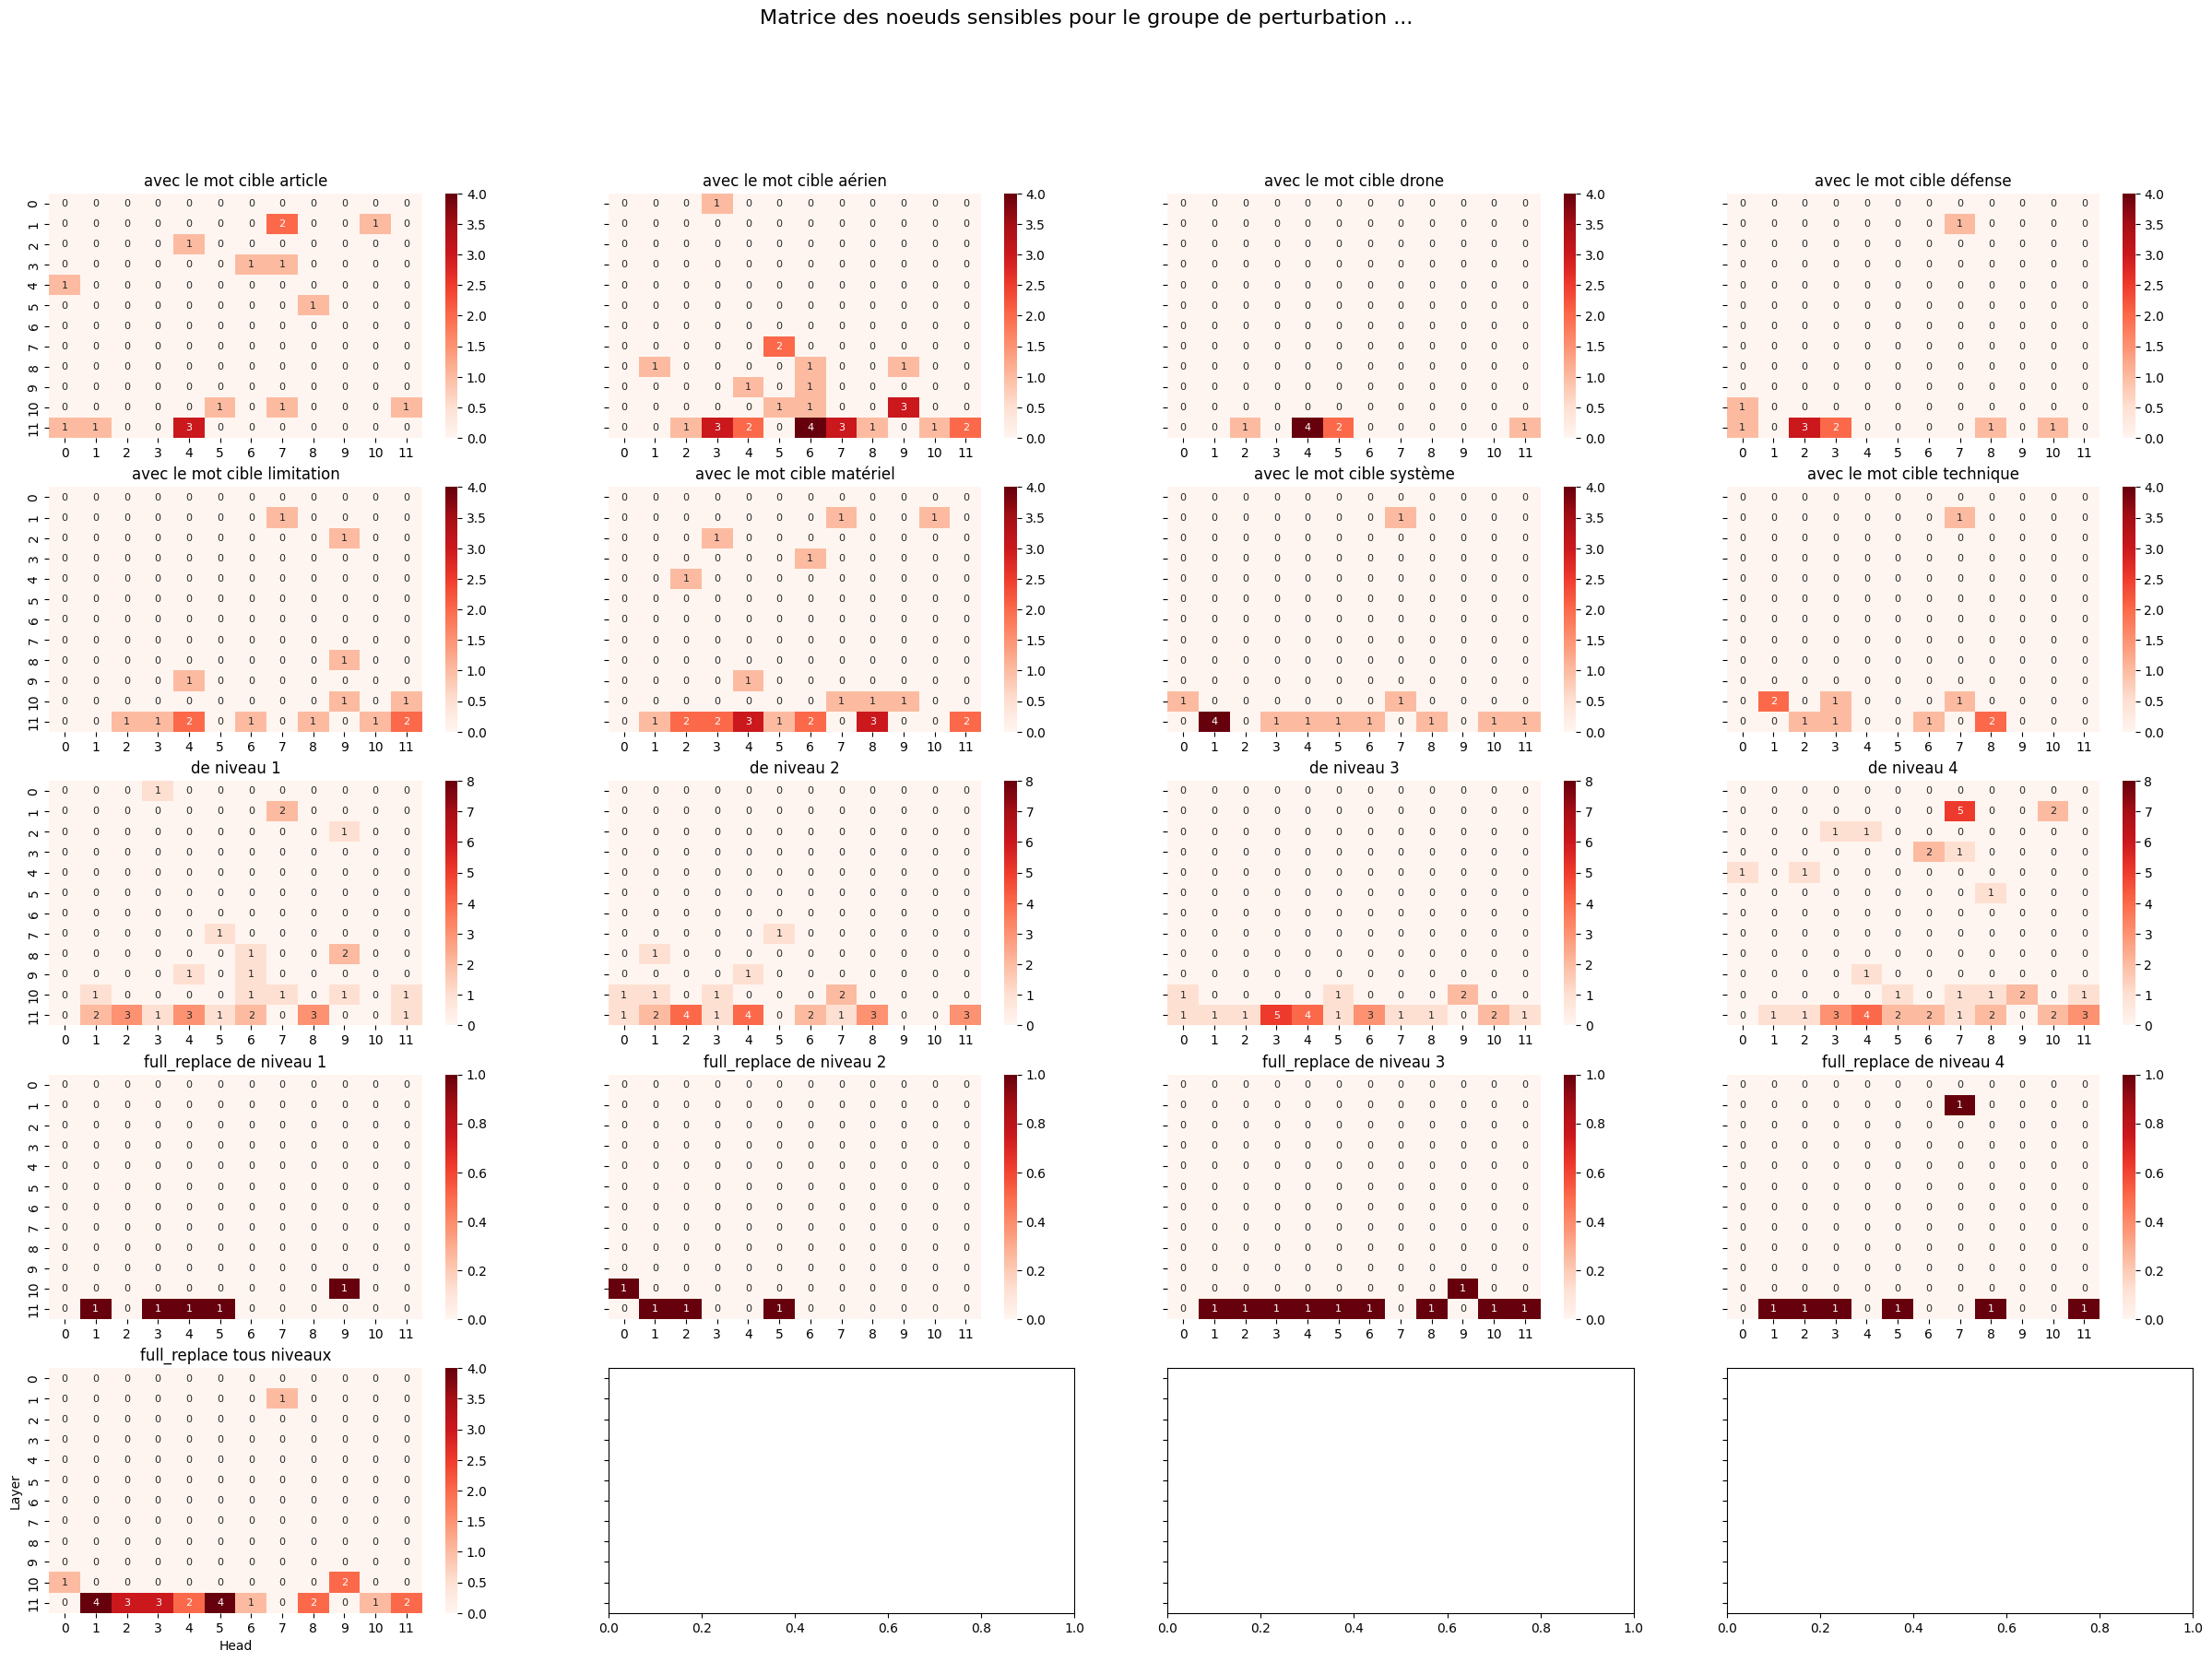
\includegraphics[width=0.8\textwidth]{images/MatriceNoeudsSensibles_all.png}
\end{frame}


\end{document}

